\chapter{Uni-Gram Distributions over Time}
\label{appendix:unigram_distributions}

Below, you can find the distribution of uni-grams extracted from the output of the model when evaluating it on the test dataset (for each snapshot), compared to the expected distributions of the same uni-grams from the training corpus. They are used in the Chapter~\ref{results:development_language_model}.

\section{OpenSubtitles}
\begin{figure}[H]
  \minipage{0.5\textwidth}
  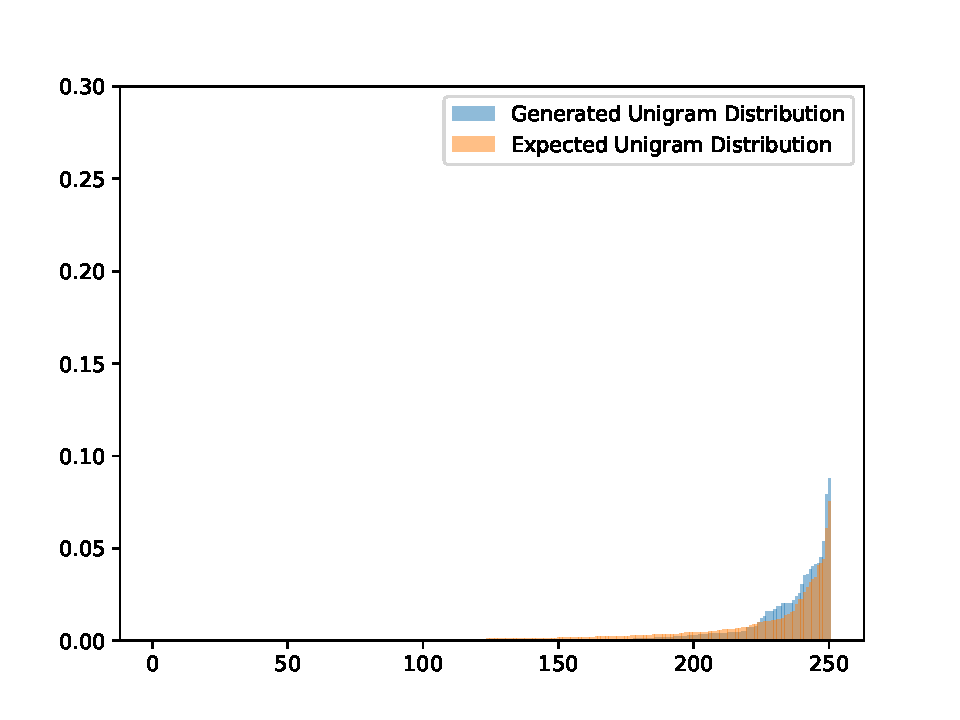
\includegraphics[width=\linewidth]{img/plots/opensubtitles_not_reversed/unigram_distribution_comparison_step_500000.pdf}
  \centering
  \small
  \text{Snapshot 0.5M}
  \endminipage\hfill
  \minipage{0.5\textwidth}
  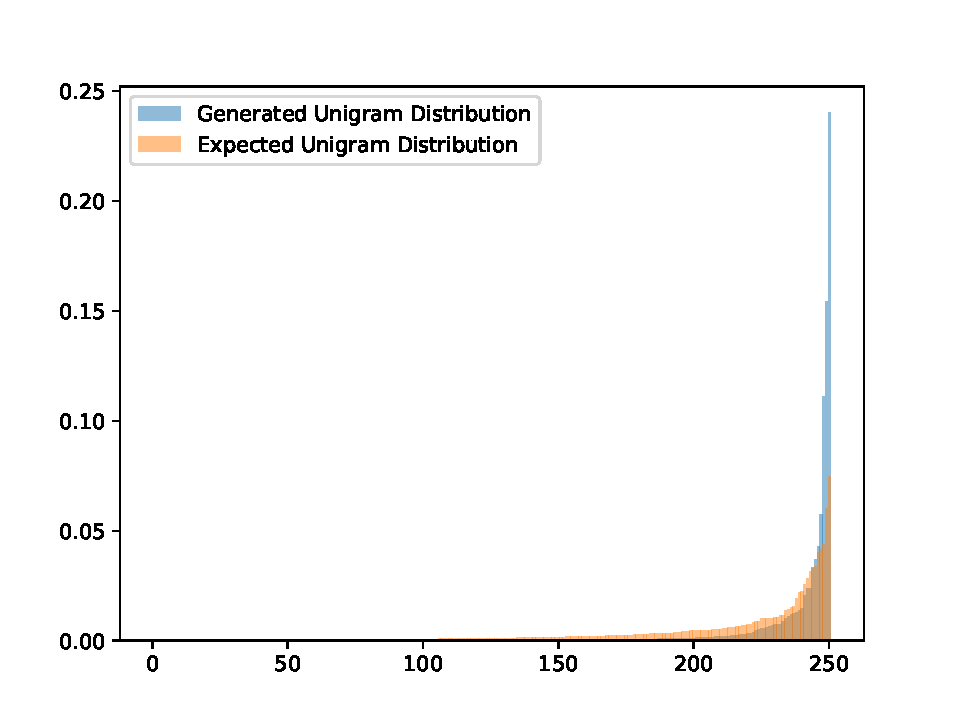
\includegraphics[width=\linewidth]{img/plots/opensubtitles_not_reversed/unigram_distribution_comparison_step_1000000.pdf}
  \centering
  \small
  \text{Snapshot 1.0M}
  \endminipage\hfill
  \minipage{0.5\textwidth}
  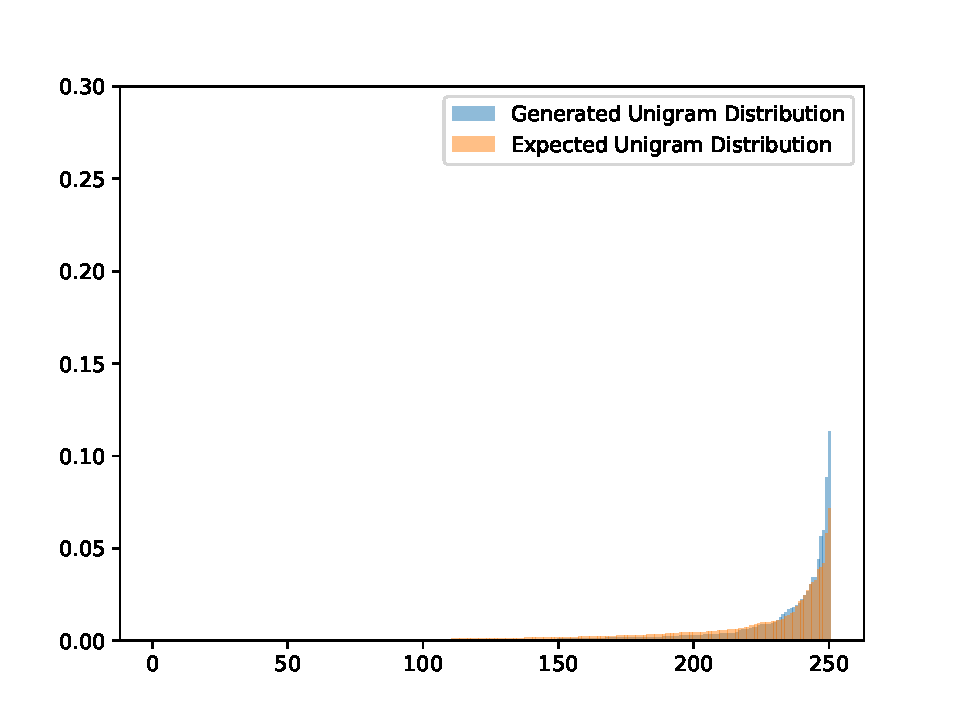
\includegraphics[width=\linewidth]{img/plots/opensubtitles_not_reversed/unigram_distribution_comparison_step_1500000.pdf}
  \centering
  \small
  \text{Snapshot 1.5M}
  \endminipage\hfill
  \minipage{0.5\textwidth}
  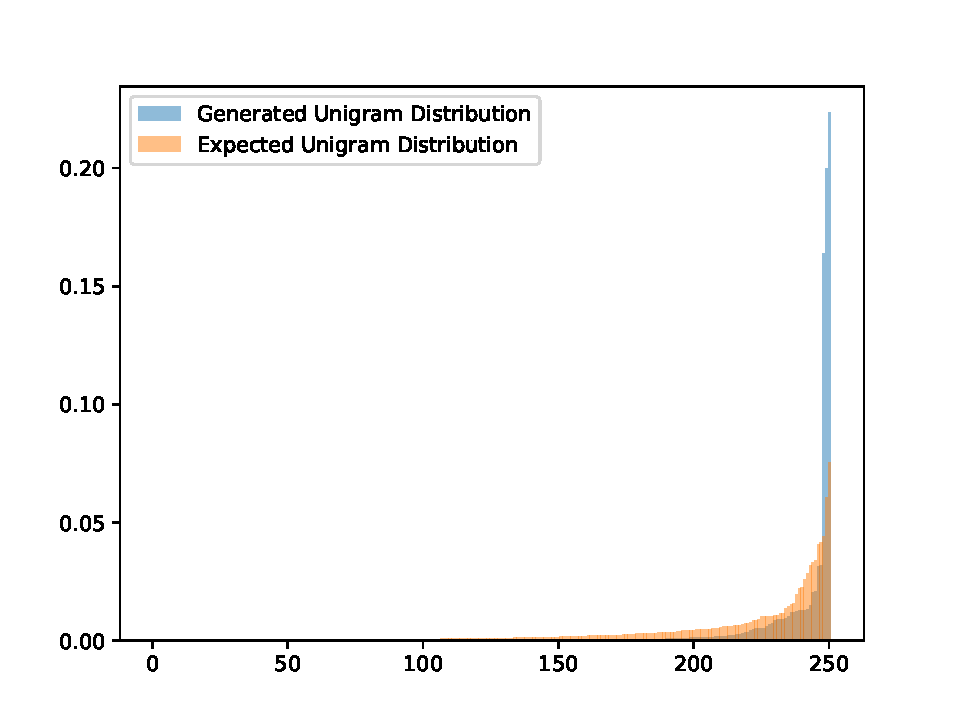
\includegraphics[width=\linewidth]{img/plots/opensubtitles_not_reversed/unigram_distribution_comparison_step_2000000.pdf}
  \centering
  \small
  \text{Snapshot 2.0M}
  \endminipage\hfill
  \minipage{0.5\textwidth}
  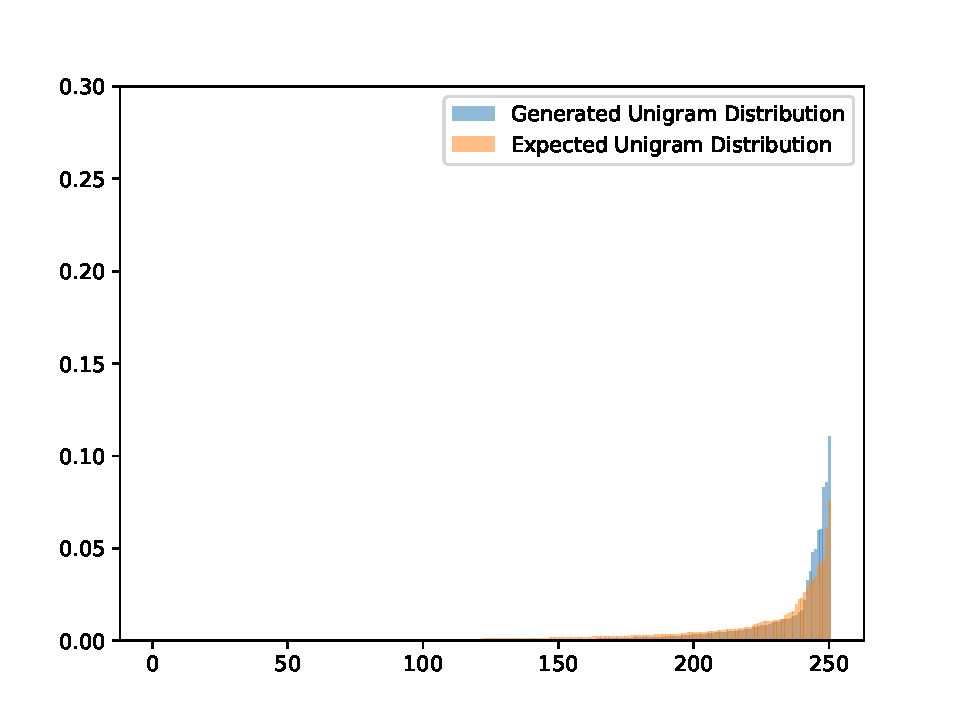
\includegraphics[width=\linewidth]{img/plots/opensubtitles_not_reversed/unigram_distribution_comparison_step_2500000.pdf}
  \centering
  \small
  \text{Snapshot 2.5M}
  \endminipage\hfill
  \minipage{0.5\textwidth}
  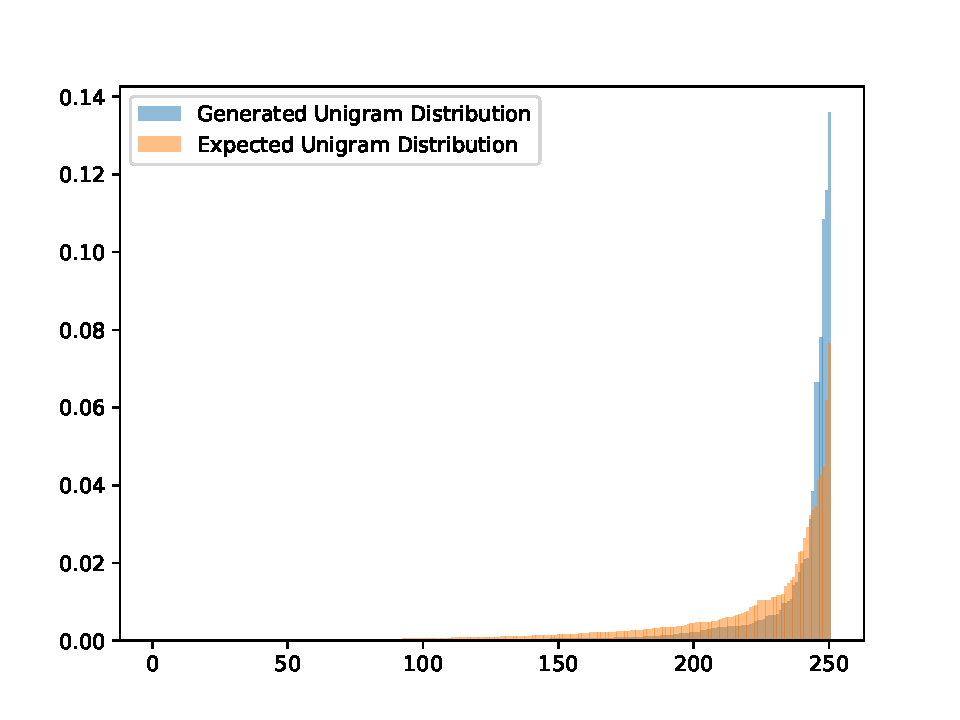
\includegraphics[width=\linewidth]{img/plots/opensubtitles_not_reversed/unigram_distribution_comparison_step_3000000.pdf}
  \centering
  \small
  \text{Snapshot 3.0M}
  \endminipage\hfill
  \caption{Comparison of the distributions of the top 100 most used unigrams for the responses of the OpenSubtitles models (orange) when using the test dataset and the distribution within the training data (blue). The distributions are compared for each snapshot available.}
  \label{results:unigram:distributions:opensubtitles}
\end{figure}

\section{Reddit}
\begin{figure}[H]
  \minipage{0.5\textwidth}
  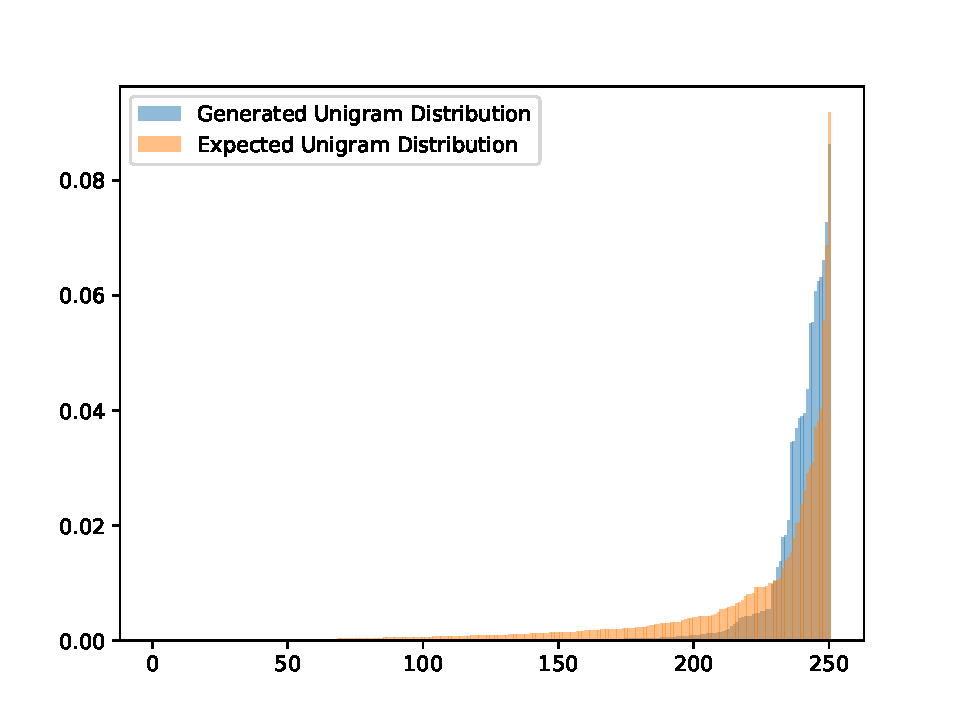
\includegraphics[width=\linewidth]{img/plots/reddit/unigram_distribution_comparison_step_500000.pdf}
  \centering
  \small
  \text{Snapshot 0.5M}
  \endminipage\hfill
  \minipage{0.5\textwidth}
  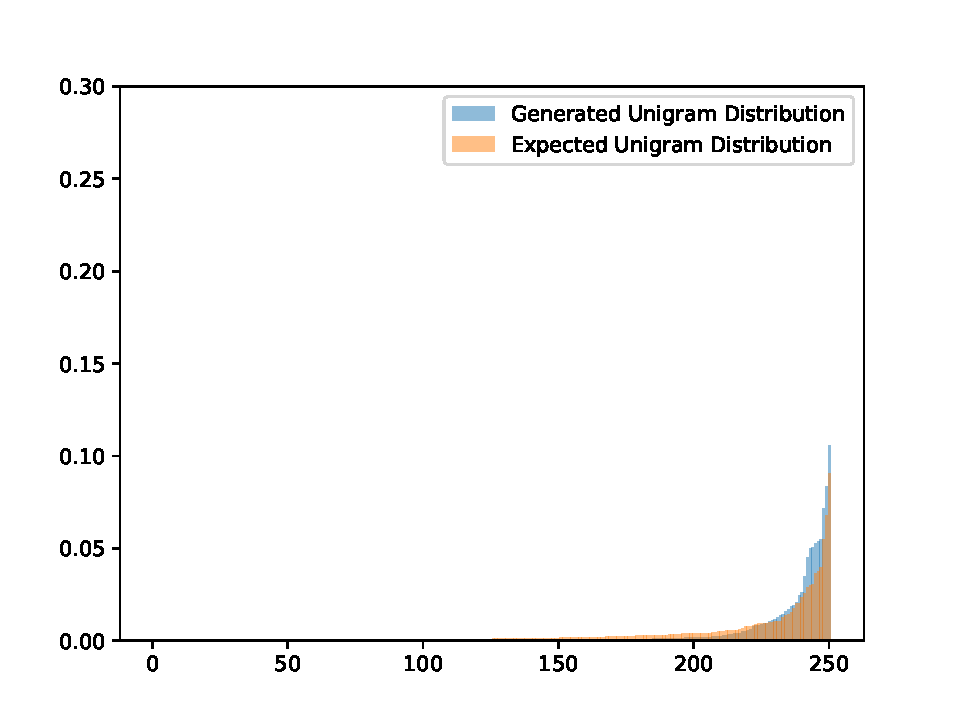
\includegraphics[width=\linewidth]{img/plots/reddit/unigram_distribution_comparison_step_1000000.pdf}
  \centering
  \small
  \text{Snapshot 1.0M}
  \endminipage\hfill
  \minipage{0.5\textwidth}
  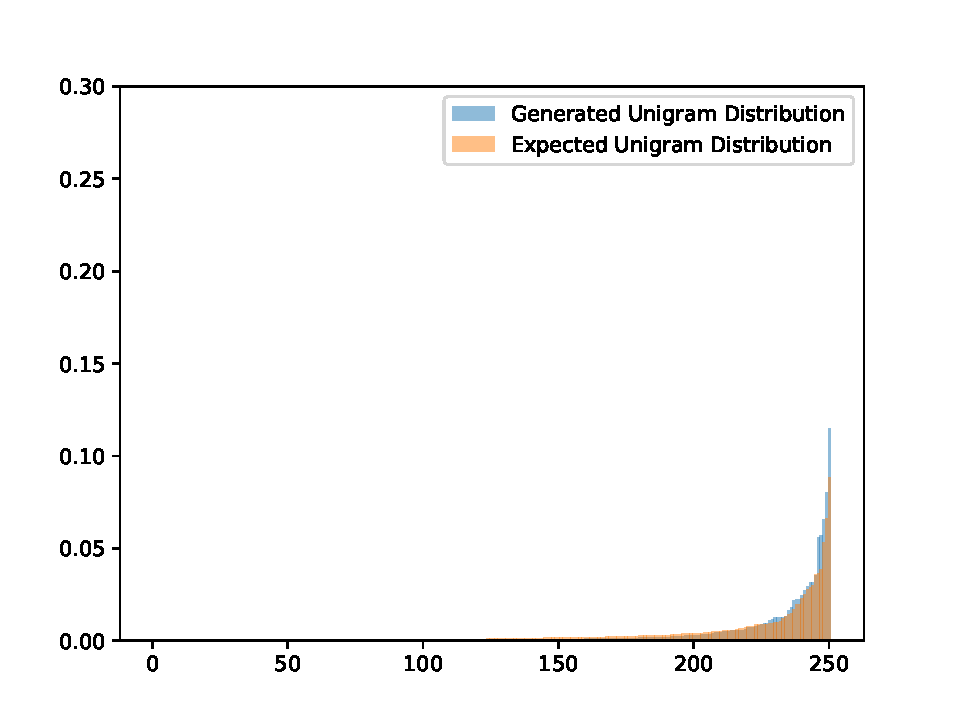
\includegraphics[width=\linewidth]{img/plots/reddit/unigram_distribution_comparison_step_1500000.pdf}
  \centering
  \small
  \text{Snapshot 1.5M}
  \endminipage\hfill
  \minipage{0.5\textwidth}
  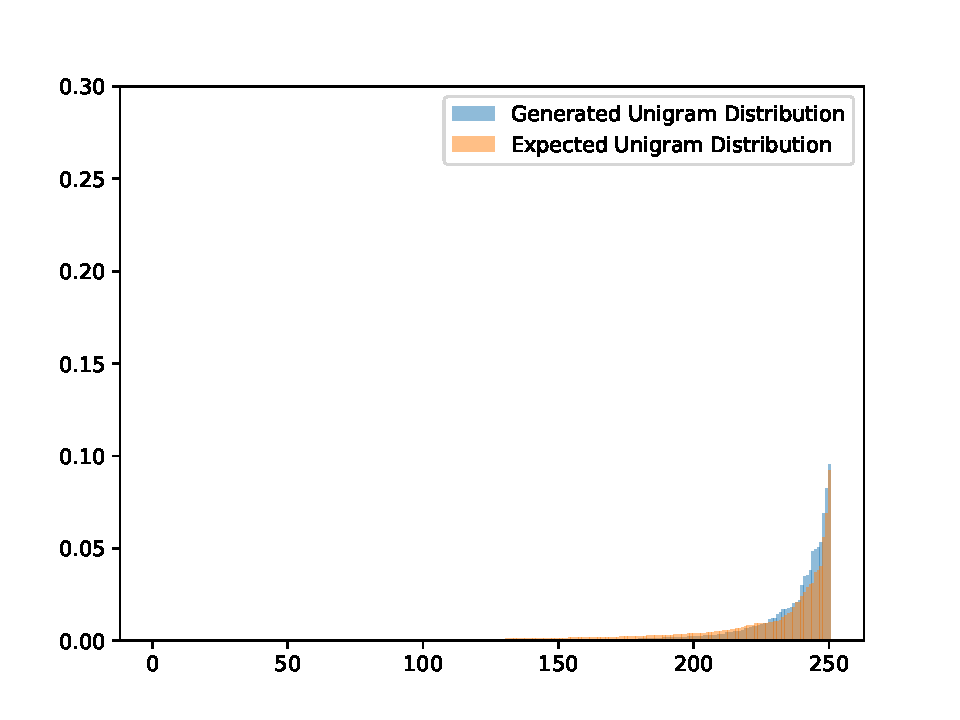
\includegraphics[width=\linewidth]{img/plots/reddit/unigram_distribution_comparison_step_2000000.pdf}
  \centering
  \small
  \text{Snapshot 2.0M}
  \endminipage\hfill
  \minipage{0.5\textwidth}
  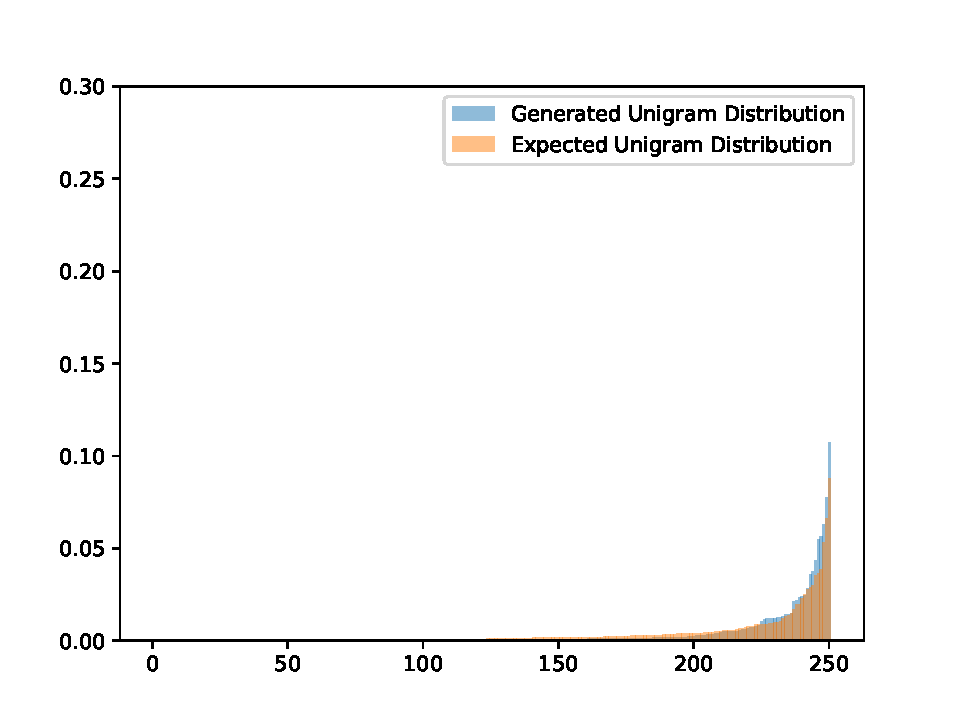
\includegraphics[width=\linewidth]{img/plots/reddit/unigram_distribution_comparison_step_2500000.pdf}
  \centering
  \small
  \text{Snapshot 2.5M}
  \endminipage\hfill
  \minipage{0.5\textwidth}
  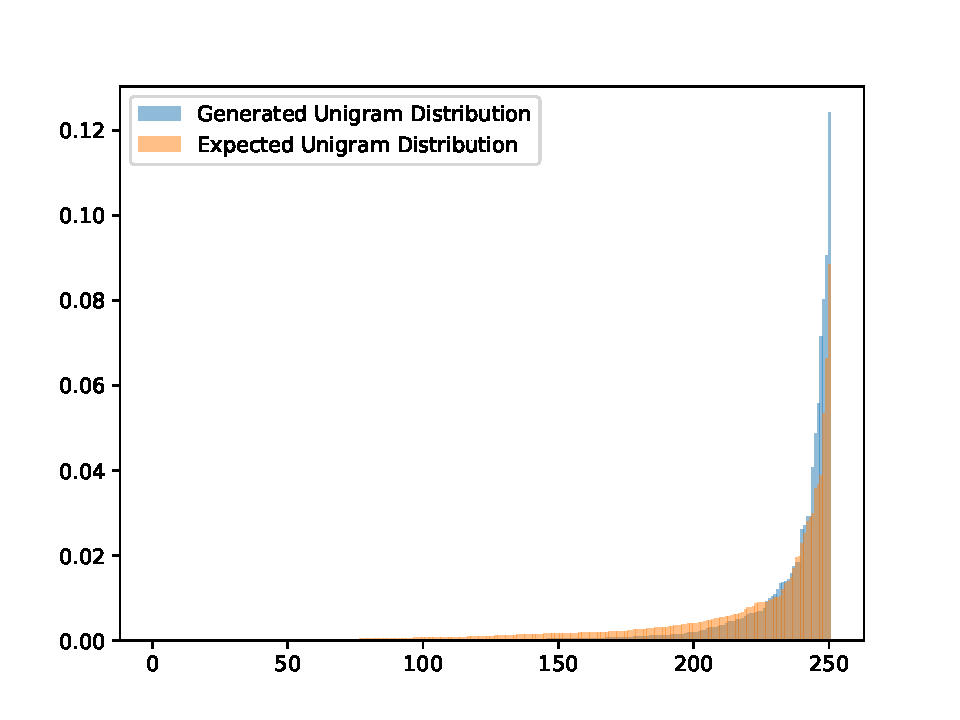
\includegraphics[width=\linewidth]{img/plots/reddit/unigram_distribution_comparison_step_3000000.pdf}
  \centering
  \small
  \text{Snapshot 3.0M}
  \endminipage\hfill
  \caption{Comparison of the distributions of the top 100 most used unigrams for the responses of the Reddit models (orange) when using the test dataset and the distribution within the training data (blue). The distributions are compared for each snapshot available.}
  \label{results:unigram:distributions:reddit}
\end{figure}